\chapter{Shrinkage metoder}
I dette kapitel vil vi finde $\widehat\lambda$, som giver den bedste model for de forskellige shrinking metoder. 
Vi har introduceret to algoritmer til at løse vores optimeringsproblemer, som vi vil anvende.
Vi deler derfor vores analyse op i to dele  hhv. coordinate descent og LARS algoritmen.
Herunder finder vi så  $\widehat\lambda$ ved hjælp af 10-fold krydsvalidering og BIC. 
Krydsvalidering bliver målt  i gennemsnitlige kvadrerede fejl, hvor vi er interesseret den model med mindst gennemsnitlige kvadrerede fejl, men hvor kompleksiteten også spiller en rolle.
Idet vi ikke kun ser på den $\lambda$ der giver mindst mulige krydsvaliderings fejl (der betegnes $\lambda_{\min}$), men også den største værdi således at fejlen er indenfor en standard afvigelse af minimum, som vi betegner $\lambda_{\text{1sd}}$.  

BIC er defineret i definition \ref{def:bic}, hvor i kompleksiteten er inkluderet i et strafparameter. Så vi er kun interesseret i den model med mindst BIC. 

\section{Coordinate descent}
I dette afsnit vil vi finde tuning parameteren $\widehat\lambda$, som giver den optimale model for lasso og dens generaliseringer. 
Hertil anvendes funktionen \texttt{glmnet} fra \Rlang-pakken af samme navn til at estimere parametrene af hver model. 
Funktionen genererer ud fra træningsmængden en følge med 100 værdier af $\lambda$, og fitter en model til hver af disse ved maksimum likelihood estimation med algoritmen coordinate descent. 

For group lasso har vi anvendt funktionen \texttt{gglasso} fra \Rlang-pakken også med samme navn til at estimere parametrene for group lasso. 
Denne funktion generer også en følge med 100 værdier af $\lambda$, men anvender i stedet algoritmen block-wise descent. 
Funktionen kræver at variablerne er opdelt i grupper, hvortil vi betragter grupperne som er forslået af Michael McCracken, som ses i appendiks \ref{app:app_data}. 
Derudover har kvadratroden af gruppens størrelse som penality faktor.

Vi finder så $\widehat\lambda$ for modellerne ved hjælp af 10-fold krydsvalidering og BIC. 

Det skal lige bemærkes, at for elastisk net har vi to turning parameter vi skal estimerer nemlig $\alpha$ og $\lambda$.  Så her har vi valgt 10 værdier af $\alpha$, hvor $\alpha \in (0,1)$. 

For adaptive lasso med lasso vægte, anvender vi kun de forklarende variable, som lasso har udvalgt til at estimerer turning parameteren $\lambda$. 

I kapitel \ref{kap:statistisk_inferens} introducerede vi for inferens for lasso modellen, hvor lambda er fast.
Til det anvender vi funktionen  \texttt{fixedLassoInf} fra \Rlang-pakken \texttt{selectiveInference} (ses i appendiks ...) 
Funktionen udregner \(p\)-værdier og konfidensintervaller for lasso estimatet for en fast værdi af tuning parameteren.
Funktionen kan dog kun anvendes af lasso og ikke dens generaliseringer. 

\subsection{Krydsvalidering}
Funktionerne \texttt{cv.glmnet} og \texttt{cv.gglasso} fra pakkerne \texttt{glmnet} og \texttt{gglasso} udfører 10-fold krydsvalidering.

Figur \ref{fig:cv_plot} illustrerer den gennemsnitlige krydsvalideringsfejl samt øvre og nedre standardafvigelse for hver værdier af $\log \del{\lambda}$ for lasso og dens generaliseringer. 
De to lodrette stiplede linjer indikerer \(\lambda_{\text{min}}\) og \(\lambda_\text{1sd}\), hvor \(\lambda_{\text{min}}\) er værdien af \(\lambda\), som giver den mindste gennemsnitlige krydsvalideringsfejl og \(\lambda_\text{1sd}\) er den største værdi af \(\lambda\), således at fejlen er indenfor en standardafvigelse af minimum. 
For elastisk net finder vi, at $\alpha =1$ giver den mindste krydsvalideringsfejl, hvilket svarer til lasso modellen. Derfor betragter vi ikke elastik net i dette afsnit. 
Vi betragter adaptive lasso med OLS vægte og adaptive lasso med lasso vægte, hvor $\gamma = 0.5$, da den giver den mindste krydsvalidering fejl. 

\imgfigh{cv_plot.pdf}{1}{10-fold krydsvalideringsfejl som funktion af $\log \del{\lambda}$ for lasso og den generaliseringer. 
De stiplede linjer betegner \(\lambda_\text{min}\) og \(\lambda_\text{1sd}\).}{cv_plot}
%

\begin{table}
\center
\begin{tabular}{cccc | cccccc}
\toprule
 &  \multicolumn{3}{c}{Lasso} &  \multicolumn{3}{c}{Ridge}  \\ \midrule
 & værdi & MSE & p & 	værdi & MSE & p \\
 $\lambda_{\min}$ &0.0014& 0.0019 & 20 	& 0.0123 &  0.0049 & 122 \\ 
 $\lambda_{1 \text{sd}}$ & 0.0027 & 0.0020 & 15 & 0.0148 & 0.0051 & 122  \\ \bottomrule \toprule
  &  \multicolumn{3}{c}{Elastic Net}  &  \multicolumn{3}{c}{Group Lasso}  \\ \midrule
 & værdi & MSE & p & værdi & MSE & p \\
 $\lambda_{\min}$ & 0.0014 & 0.0020 & 23 & 0.0003 & 0.0023  & 122\\
  $\lambda_{1\text{sd}}$ & 0.0027 & 0.0021 & 15 & 0.0005 & 0.0024 & 122 \\  \bottomrule \toprule
 &  \multicolumn{3}{c}{Adaptive lasso m. OLS vægte}  &  \multicolumn{3}{c}{Adaptive lasso m. lasso vægte}  \\ \midrule
  & værdi & MSE & p & værdi & MSE & p \\
 $\lambda_{\min}$  & 0.0868 & 0.0018 & 2 & 0.0034 & 0.0018 & 4   \\
 $\lambda_{1\text{sd}}$ & 0.4222 & 0.0018 & 2 & 0.0085 & 0.0019 & 4  \\ \bottomrule
 \end{tabular}
\caption{Tabellen viser $\lambda$ værdierne fundet udfra krydsvalidering, samt krydsvalideringsfejl, som er målt i MSE og antallet af parameter.} \label{tab:cv_tab}
\end{table}


For at give et bedre overblik giver tabel \ref{tab:cv_tab} værdierne af $\log \del{ \lambda_{\min}}$ og $\log \del{ \lambda_{1\text{sd}}}$, krydsvalideringsfejl, antallet af parametre, justerede R$^2$ og log-likelihood for lasso og dens generaliseringer.
%Den valgte tuning parameter er markeret med tykt for hver metode.   

For lasso ses en markant reducering i antallet af parametre for $\lambda_{1\text{sd}}$ i forhold til $\lambda_{\min}$, dette øger ikke krydsvalideringsfejlen betydeligt, og derfor anvendes $\widehat{\lambda}_{1\text{sd}}$ som tuning parameter for lasso. 
Ridge regression mindsker blot koefficienterne, og derfor vælges alle variable. For ridge regression vælger vi \(\lambda_{\min}\) som tuning parameter, da den har mindst krydsvalideringsfejl.
For group lasso vælges lidt overraskende alle parametre med \(\lambda_\text{min}\), mens antallet af parametre reduceres med 7 for $\lambda_{1\text{sd}}$. 
Disse 7 variable tilhører alle gruppe 5.
Vi lader $\widehat{\lambda}_{1\text{sd}}$ være den optimale tuning parameter for group lasso, da den har det færreste antal parametre.
Adaptive lasso med OLS vægte og lasso vægte vælger blot to variable for både \(\lambda_\text{min}\) og \(\lambda_{1\text{sd}}\).
Vi lader $\lambda_{1\text{sd}}$ være tuning parameteren for adaptive lasso modellerne.  
De valgte model---

Justerede R\(^2\) er størst for adaptive lasso modellerne og mindst for ridge regression.
%
%
%For lasso ses en markant reducering i antallet af parametre for $\lambda_{1\text{sd}}$ i forhold til $\lambda_{\min}$. Dette øger ikke krydsvalideringsfejlen eller justerede R$^2$ betydeligt, og derfor anvendes $\widehat{\lambda}_{1\text{sd}}$ som tuning parameter for lasso. 
%Vi ser også, at ridge regression har den mindste værdi af justerede R$^2$ samt den højeste værdi af log-likelihood, men modellen mindsker også blot koefficienterne. 
%For ridge regression vælger vi, derfor $\widehat{\lambda}_{\min}$ som tuning parameter, da den har mindst krydsvalideringsfejl.
%
%For group lasso vælges lidt overraskende alle parametre med \(\lambda_\text{min}\), mens antallet af parametre reduceres med 7 for $\lambda_{1\text{sd}}$. 
%Disse 7 variable tilhører alle gruppe 5.
%Vi anvender $\widehat{\lambda}_{1\text{sd}}$ som turning parameter, da den har færreste antal parametre. 
%Adaptive lasso m. OLS vægte og lasso vægte vælger blot to variable for $\lambda_{1\text{sd}}$ uden at det øger deres krydsvalideringsfejl betydeligt. 
%Derfor lader vi $\lambda_{1\text{sd}}$ være tuning parameteren for adaptive lasso modellerne. 

På figur \ref{fig:coef_kryds_coord} vises de 14 estimerede koefficienter for lasso og de 2 estimerede koefficienter for adaptive lasso.

Heraf ses, at lasso hovedsagligt vælger variable i samme gruppe som arbejdsløshedsraten.
For lasso ses at variablerne valgt af adaptive lasso, \textcolor{blue3}{CLF16OV} og \textcolor{blue3}{CE16OV}, har de største estimerede koefficienter, efterfulgt af \textcolor{blue3}{UEMPLT5}, \textcolor{blue3}{UEMP5TO14}, \textcolor{blue3}{UEMPL15OV} og \textcolor{blue3}{lag 1}, mens de øvrige er meget tæt på nul. 
Figur \ref{fig:coef_ridge_kryds_coord} og \ref{fig:coef_gglasso_kryds_coord} viser de estimerede koefficienter for henholdsvis ridge regression og group lasso.
Igen ser vi, at variablerne \textcolor{blue3}{CLF16OV} og \textcolor{blue3}{CE16OV} klart har de største estimerede koefficienter.    
%
\imgfigh{coef_kryds_coord.pdf}{1}{Estimerede koefficienter for lasso og adaptive lasso med OLS og lasso vægte,  hvor $\widehat{\lambda}$ er fundet ud fra krydsvalidering.
Farverne indikerer hvilken gruppe, variabler tilhører, og y-aksen er variablerne udvalgt af lasso. }{coef_kryds_coord}


Figur \ref{fig:resid_lasso_coord_kryds}-\ref{fig:resid_adap_ols_coord_kryds} viser en analyse af de standardiserede residualer for lasso og dens generaliseringer. 
Vi ser, samme tendens for lasso og dens generaliseringer. Histogrammet og QQ-plottet indikerer tungere haler end normalfordelingen og autokorrelation i første lag.
Dette bekræftes i tabel \ref{tab:res_shrinkage_tab}, som viser skewness, excess kurtosis, $p$-værdier fra JB-testen og LB testen for de standardiserede residualer, hvor $\widehat{\lambda}$ er estimerede udfra krydsvalidering.  
Vi ser, at alle modellerne har en negativ skewness og en kurtosis forskellige fra nul. 
Derudover afvises JB testens nulhypotesen om normalitet for alle modeller med undtagelse af group lasso, dog har den en lille skewness og kurtosis.
For LB testen afvises nulhypotesen om uafhængighed for alle modeller.

\subsubsection{Inferens}
På figur \ref{fig:boxplot_lasso_coord_kryds} ses bootstrap resultater for variablene udvalgt af lasso.
Da adaptive lasso har konsistent variabeludvælgelse, vil variablerne \textcolor{blue3}{CLF16OV} og \textcolor{blue3}{CE16OV} altid vælges, derfor laves der ikke bootstrap for disse.
Variablerne \textcolor{orange}{TB6MS}, \textcolor{blue3}{PAYEMS} og \textcolor{red3}{DPCERA3M086SBEA} fravælges over 50\% af bootstrap realisationerne, mens variablerne  \textcolor{blue3}{lag 1}, \textcolor{blue3}{UEMPL15OV}, \textcolor{blue3}{UEMP5TO14}, \textcolor{blue3}{UEMPLT5}, \textcolor{blue3}{CE16OV} og \textcolor{blue3}{CLF16OV} ofte vælges.
Generelt fravælges variablerne, som ikke tilhører gruppe 2.
I forhold til størrelsen af de estimerede koefficienter for lasso er bootstrap resultaterne ikke overraskende. 

Herefter anvendes TG testen for lasso modellen.
Resultaterne er givet i tabel \ref{tab:fixedLassoInf}.
Heraf ser vi at variablerne \textcolor{blue3}{CLF16OV}, \textcolor{blue3}{CE16OV} og \textcolor{blue3}{lag 1} afviser nulhypotesen, og derfor er signifikante.
$Z$-score er udregnet for $s_k \boldsymbol{\eta}^T \textbf{y}$, hvor $s_k$ er fortegnet for den $k$'te variable. 
Vi observerer, at $Z$-score er meget stor for variablerne \textcolor{blue3}{CLF16OV} og \textcolor{blue3}{CE16OV}, mens den er relative lav for de resterende variabler. 
Vi ser også, at  $\mathcal{V^-} \leq \boldsymbol{\eta}^T \textbf{y} \leq \mathcal{V^+}$, som stemmer overens med teorien.
%
%\imgfigh{ols_lasso_interval_kryds.pdf}{1}{ }{ }

%
\begin{table}[h] 
\centering 
\scalebox{0.8}{
\begin{tabular}{llllllll}
\toprule
Prædiktor & Koefficient & Z-score & \(p\)-værdi & lowConfPt & UpConfPt & LowTailArea & UpTailArea\\
\midrule
\textcolor{red3}{DPCERA3M086SBEA} & -0.002 & -1.365 &  0.666  &  -0.009  &  0.026   &    0.050   &   0.050 \\
\textcolor{chartreuse4}{IPDMAT} & -0.003  &-1.113  & 0.268  &  -0.012 &   0.006    &   0.050    &  0.049 \\
\textcolor{blue3}{HWIURATIO}  & 0.002 &  0.718 &  0.197 &   -0.003 &   0.014  &     0.049  &    0.050 \\
\textcolor{blue3}{CLF16OV} & 0.243 & 36.668  & 0.000   &  0.232  &  0.259     &  0.049  &    0.049 \\
\textcolor{blue3}{CE16OV} &  -0.266 & -37.390 &  0.000  &  -0.280 &  -0.254   &    0.049  &    0.049\\
\textcolor{blue3}{UEMPLT5} & 0.001  & 0.241  & 0.402  &  -0.005  &  0.008     &  0.049   &   0.049\\
\textcolor{blue3}{UEMP5TO14} & 0.000 & -0.118 &  0.429  &  -0.007  &  0.004   &    0.049  &    0.049\\
\textcolor{blue3}{UEMP15OV}& 0.004  & 1.593  & 0.056 &    0.000  &  0.009  &     0.049    &  0.050 \\
\textcolor{blue3}{PAYEMS} & 0.001 &  0.273  & 0.223  &  -0.007  &  0.029     &  0.050   &   0.050 \\
\textcolor{blue3}{USCONS} & -0.002 & -0.883 &  0.569 &   -0.009  &  0.016  &     0.050  &    0.000 \\
\textcolor{orange}{TB6MS} & -0.001 & -0.480 &  0.682 &   -0.009  &  0.026  &     0.050   &   0.050 \\
\textcolor{orange}{GS5} & -0.003 & -1.131  & 0.219  &  -0.025  &  0.007     &  0.050   &   0.049\\
\textcolor{orange}{EXUSUKx} & 0.003 &  1.306 &  0.872 &   -0.072  &  0.003  &     0.050  &    0.050 \\
\textcolor{blue3}{lag 1} & -0.009 & -4.067  & 0.003 &   -0.013 &  -0.004  &     0.049    &  0.049 \\
\bottomrule
\end{tabular}  
}
\caption{\(p\)-værdier og konfidensintervaller for variablerne udvalgt af lasso. Den estimeres standard afvigelse er \(0.043\), og resultaterne er for \(\lambda \approx 1.823\) med \(\alpha = 0.1\).} \label{fig:fixedLassoInf}
\end{table} 
%

\subsection{BIC}
Hernæst vil vi estimere tuning parameteren med BIC.
For elastisk net finder vi, at $\alpha = 1$ giver den mindste BIC, derfor betragter vi igen ikke elastisk net.
For adaptive lasso med OLS vægte (BIC) finder vi, at $\gamma = 2$ giver den mindste BIC, og for adaptive lasso med lasso vægte (BIC) får vi, at $\gamma = 0.5$ giver den mindste BIC. 

Tabel \ref{tab:bic_lambda} giver værdierne af $\log \del{ \lambda_\text{BIC}}$, BIC, antallet af parametre, justeret R$^2$ og log-likelihood for lasso og dens generaliseringer. 
Justeret R$^2$ er igen størst for lasso (BIC) og mindst for ridge regression (BIC).

%\begin{table}
%\center
%\begin{tabular}{lccc} 
%\toprule
%& \multicolumn{1}{c}{Lasso} & \multicolumn{1}{c}{Ridge regression}  &  \multicolumn{1}{c}{Group lasso}\\ \midrule
%$\log \del{\widehat{\lambda}_\text{BIC}}$ & $-6.2639$ & $-4.4730$  & $-7.2876$ \\
%$p$ & 17 & 126 & 99 \\
%BIC & $-6.1608 $& $-3.3230$ & $-5.0721$  \\
%Adj. R$^2$ & 94.23 \% & 86.98  \%   & 92.11 \%  \\ \bottomrule \toprule
%& Adap. lasso m. OLS vægte & Adap. lasso m. lasso vægte \\ \midrule
%$\log \del{ \widehat{\lambda}_\text{BIC}}$ &  $-2.6212$& $-1.8390$ \\
%$p$ & 2&2 \\
%BIC &  $-6.3153$&$-6.3142$ \\
%Adj. R$^2$ & 94.28 \% &  94.28 \% \\ \bottomrule
% \end{tabular}
%\caption{Logaritmen af $\widehat{\lambda}_\text{BIC}$, antallet af parametre, BIC og adjusted R$^2$ for lasso og dens generaliseringer.} \label{tab:bic_lambda}
%\end{table}

\begin{table}
\center
\begin{tabular}{lcccc  | lccccc} 
\toprule
 \multicolumn{5}{c}{Lasso} && \multicolumn{5}{c}{Ridge regression}  \\ \midrule
& $\log \del{\widehat{\lambda}_\text{BIC}}$  & BIC & $p$ & R$^2_{\text{adj}}$ && & $\log \del{\widehat{\lambda}_\text{BIC}}$  &  BIC & $p$ &R$^2_{\text{adj}}$  \\
$\widehat{\lambda}_\text{BIC} $&  $-6.2639$ & $-6.1608$ & 17 &  94.23 \% && $\widehat{\lambda}_\text{BIC} $ & $-4.4730$ & $-3.3230$ &  126 & 86.98 \% \\ \bottomrule \toprule 
 \multicolumn{5}{c}{Group lasso} && \multicolumn{5}{c}{Adap. lasso m. OLS vægte}  \\ \midrule
& $\log \del{\widehat{\lambda}_\text{BIC}}$  & BIC & $p$ &R$^2_{\text{adj}}$ && & $\log \del{\widehat{\lambda}_\text{BIC}}$  &  BIC & $p$ &R$^2_{\text{adj}}$   \\
$\widehat{\lambda}_\text{BIC}$ & $-7.2876$ &  $-5.0721$ &99  & 92.11\% &&  $\widehat{\lambda}_\text{BIC}$ & $-2.6212$ &  $-6.3153$  & 2 & $94.28 \%$ \\ \bottomrule \toprule 
 \multicolumn{5}{c}{Adap. lasso m. lasso vægte}  \\
& $\log \del{\widehat{\lambda}_\text{BIC}}$  & BIC & $p$ & R$^2_{\text{adj}}$\\
 $\widehat{\lambda}_\text{BIC}  $&  	$-1.8390$ & $-6.3142$  & 2& 94.28\% \\ \cmidrule{1-5}
 \end{tabular}
\caption{Logaritmen af $\widehat{\lambda}_\text{BIC}$, antallet af parametre, BIC og adjusted R$^2$ for lasso og dens generaliseringer.} \label{tab:bic_lambda}
\end{table}

Figur \ref{fig:coef_bic_coord} vises de 17 estimerede koefficienter for lasso (BIC), 2 estimerede koefficienter for adaptive lasso med OLS vægte (BIC) og 3 estimerede koefficienter for adaptive lasso med lasso vægte (BIC).
Adaptive lasso med OLS vægte (BIC) vælger variablerne \textcolor{blue3}{CLF16OV} og \textcolor{blue3}{CE16OV}, mens adaptive lasso med lasso vægte (BIC) yderligere vælger variablen \textcolor{blue3}{lag1}. 
Igen har variablerne \textcolor{blue3}{CLF16OV} og \textcolor{blue3}{CE16OV} de største estimerede koefficienter, mens de resterende estimerede koefficienter er meget tæt på nul. 
Vi har valgt ikke at inkludere de estimerede koefficienter for ridge regression (BIC) og group lasso (BIC), da det samme gør sig gældende for disse.

\imgfigh{coef_bic_coord.pdf}{1}{Estimerede koefficienter for lasso (BIC), adaptive lasso med OLS vægte (BIC) og adaptive lasso med lasso vægte (BIC). 
Farverne indikerer hvilken gruppe, variablerne tilhører og y-aksen er variablerne udvalgt af lasso (BIC).}{coef_bic_coord}

Figur \ref{fig:resid_lasso_coord_bic}-\ref{fig:resid_adap_lasso_coord_bic} viser en analyse af de standardiserede residualer for lasso og dens generaliseringer.
For lasso (BIC), adaptive lasso med OLS vægte (BIC) og adaptive lasso med lasso vægte (BIC) observeres udfra histogrammet og QQ-plottet, at fordelingen af de standardiserede residualer har tungere haler end normalfordelingen.
For ridge regression (BIC) og group lasso (BIC) er der blot få outliers fra normalfordelingen i QQ-plottet.
Fælles for alle er, at der er autokorrelation i det første lag. 
I tabel \ref{tab:res_shrinkage_tab} afvises residualerne at være uafhængige og JB testens nulhypotese om normalitet afvises også for alle med undtagelse af group lasso (BIC).

Figur \ref{fig:boxplot_lasso_coord_bic} viser bootstrap resultaterne for variablerne udvalgt af lasso (BIC).
Variablene \textcolor{cadetblue2}{CPIMEDSL}, \textcolor{orange}{TB6MS}, \textcolor{blue3}{USTRADE} og \textcolor{blue3}{CLAIMSx} fravælges over 50\% af bootstrap realisationerne, mens variablerne \textcolor{blue3}{lag 1}, \textcolor{blue3}{UEMPL15OV}, \textcolor{blue3}{UEMPLT5}, \textcolor{blue3}{CE16OV} og \textcolor{blue3}{CLF16OV} ofte vælges.
I forhold til størrelsen af de estimerede koefficienter for lasso (BIC) er bootstrap resultaterne ikke overraskende. 
Som nævnt tidligere har adaptive lasso konsistent variabeludvælgelse og derfor laves der ikke bootstrap for adaptive lasso med OLS vægte (BIC) og adaptive lasso med lasso vægte (BIC). 

\subsubsection{TG testen}
Vi lader igen $\boldsymbol{\eta} = s_k \del{\textbf{X}^+_{\mathcal{A}_k}}^T \mathbf{e}_k$, da er $\mathcal{H}_0: \beta_k = 0$ jævnfør \eqref{eq:tg_beta}. 
Resultaterne for TG testen er givet i tabel \ref{tab:fixedLassoInf_bic}.
Heraf ser vi at variablerne \textcolor{blue3}{CLF16OV} og \textcolor{blue3}{CE16OV} afviser nulhypotesen, og derfor er signifikante.
Vi observerer et $\infty$ i den øvre grænse i konfidensintervallet for \textcolor{blue3}{USTRADE}, hvilket skyldes at konfidensintervallet er udregnet numerisk, og bliver ustabil når punktet $\boldsymbol\eta^T \mathbf{y}$ er for tæt på dens trunkerede interval, altså $\mathcal{V}^-$ og $\mathcal{V}^+$. 
Igen observeres at $Z$-score for variablerne \textcolor{blue3}{CLF16OV} og \textcolor{blue3}{CE16OV} er høje i forhold de resterende. 

Figur \ref{fig:resid_tg_bic} viser en analyse af de standardiserede fejl for lasso$_{TG}$ (BIC). Vi ser, at QQ-plottet indikerer tungere haler end normalfordeling og autokorrelation i de to første lags. 
Dette bekræftes også i tabel \ref{tab:res_shrinkage_tab}.
\begin{table}[h] 
\centering 
\scalebox{0.8}{
\begin{tabular}{llllllll}
\toprule
Prædiktor & Koefficient & Z-score & \(p\)-værdi & lowConfPt & UpConfPt & LowTailArea & UpTailArea\\
\midrule
\textcolor{red3}{DPCERA3M086SBEA}  & -0.002  &-0.960   &0.093  &   -0.071  &  0.003      & 0.000   &  0.050 \\
\textcolor{chartreuse4}{IPDMAT} &-0.002 & -0.680 &  0.159  &  -0.032 &   0.005     &  0.050    &  0.049 \\
\textcolor{blue3}{CLF16OV} & 0.241  &36.686  & 0.000 &    0.235   & 0.350    &   0.050  &    0.050 \\
\textcolor{blue3}{CE160V} &-0.264& -37.339   &0.000  &  -0.455  & -0.260   &    0.050   &   0.050 \\
\textcolor{blue3}{UEMPLT5}  & 0.000 &  0.027 &  0.777   & -0.029    &0.005    &   0.000  &     0.048 \\
\textcolor{blue3}{UEMP5TO14} & -0.001  & -0.266 & 0.599  & -0.007   &  0.014    &   0.050 &      0.050 \\
\textcolor{blue3}{UEMP15OV} &0.004  & 1.299  & 0.249   & -0.005   & 0.008  &     0.050     & 0.049 \\
\textcolor{blue3}{CLAIMSx} & 0.001 &  0.387  & 0.689   & -0.030   & 0.011    &  0.050     & 0.050 \\
\textcolor{blue3}{USCONS}  & -0.001  &  -0.591   &  0.100  &    -0.088  &     0.004  &      0.050  &       0.050 \\
\textcolor{blue3}{USTRADE}  & 0.000  & -0.118  &  0.988     & 0.007     &  Inf     &   0.050  &     0.000\\
\textcolor{red3}{AMDMNOx} &-0.002 &  -0.813 &  0.641  &  -0.008  &  0.020   &    0.049      &0.050 \\
\textcolor{orange}{TB6MS}&-0.001  &-0.415  & 0.677   & -0.008  &  0.023   &    0.049   &   0.000 \\
\textcolor{orange}{GS5} &-0.003 & -1.207  & 0.144    &-0.032  &  0.005      & 0.050    &  0.050 \\
\textcolor{orange}{EXUSUKx} & 0.003  & 1.449   &0.303   & -0.007   & 0.012      & 0.050    &  0.050 \\
\textcolor{cadetblue2}{CPIMEDSL}  &0.002 &  0.855 &  0.865&    -0.054 &   0.003&       0.050    &  0.050 \\
\textcolor{blue3}{lag1} & -0.010&  -4.362 &  0.499  &  -0.011   & 0.033   &    0.050  &    0.050 \\
\textcolor{blue3}{lag4}  & 0.002 &   1.106   & 0.311    & -0.014 &    0.028 &       0.036 &      0.050 \\
\bottomrule
\end{tabular}  
}
\caption{\(p\)-værdier og konfidensintervaller for variablerne udvalgt af lasso med BIC. Den estimeres standard afvigelse er 0.043, og resultaterne er for $\lambda \approx 1.0432$  med \(\alpha = 0.1\).} \label{tab:fixedLassoInf_bic}
\end{table} 








\section{LARS}
\begin{frame}{LARS}
\begin{itemize}
\item Fitter en model for hvert trin
\begin{itemize}
\item LARS algoritmen foretager 127 trin 
\item LARS algoritmen med lasso modifikationen udfører 192 trin 
\end{itemize}
\item Igen anvendes krydsvalidering og BIC til at estimere tuning parameteren, som for LARS algoritmen er fraktionen af \(\ell_1\)-normen \(f = \frac{\vert \boldsymbol{\beta} \vert}{\max \vert \boldsymbol{\beta} \vert}\), hvor \(f \in \sbr{0,1}\).
\begin{itemize}
\item \(f = 0\): ingen variabler tilføjet til den aktive mængde
\item \(f = 1\): alle variable inkluderet
\end{itemize}
\end{itemize}
\end{frame}

\subsection{Krydsvalidering}
%%%%%%%% Krydsvalidering %%%%%%%%%

\begin{frame}{LARS}{Krydsvalidering}
\begin{figure}
 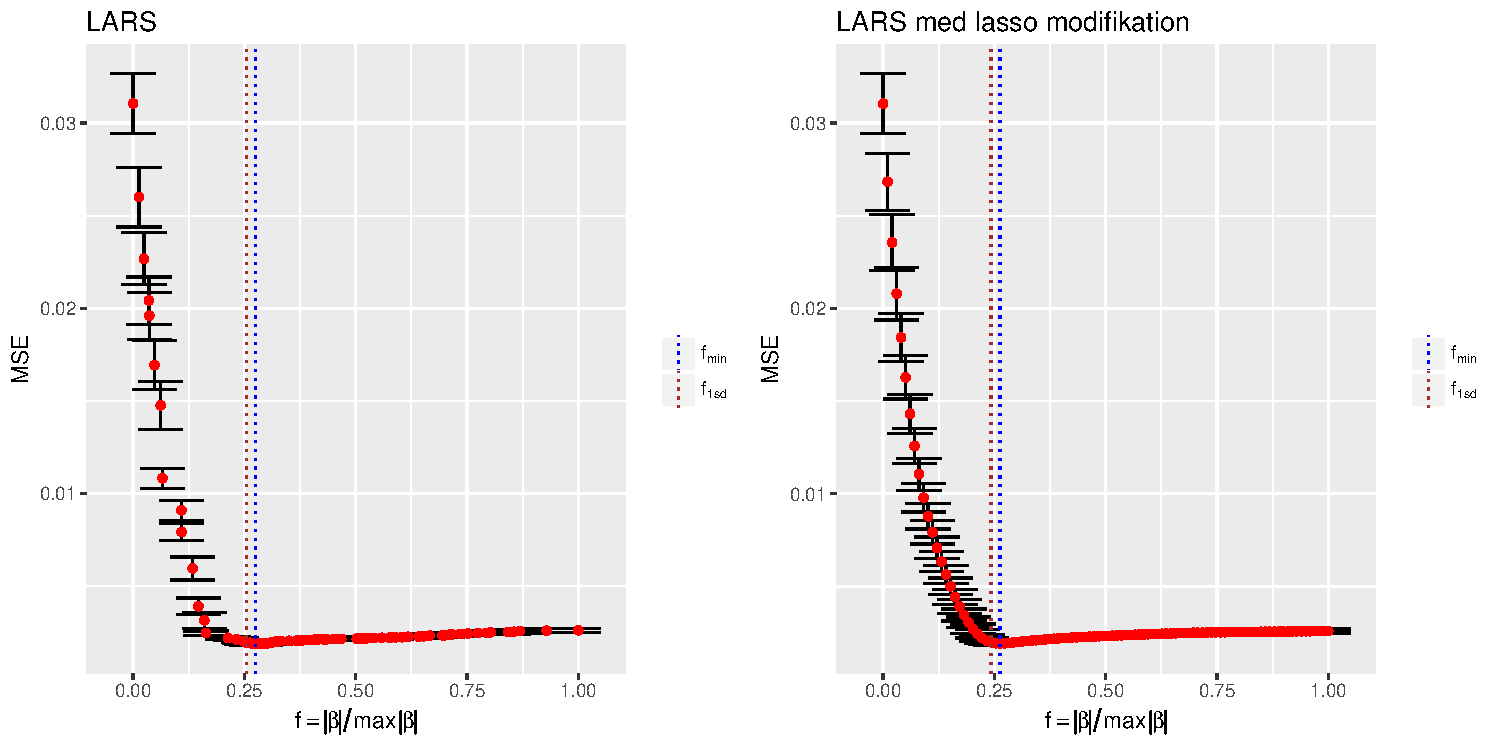
\includegraphics[width=1\linewidth, height=0.7\textheight]{slides/lars_kryds.pdf}
 \caption{10-fold krydsvalideringsfejl som funktion af fraktionen af \(\ell_1\)-normen LARS og lasso LARS.}
 \end{figure}
 %De stiplede linjer indikerer \(f_\text{min}\) og \(f_\text{1sd}\).
\end{frame}


\begin{frame}{LARS}{Krydsvalidering}
\begin{table}
\center
\scalebox{0.8}{
\begin{tabular}{lccccc | lccccc}
\toprule
 \multicolumn{6}{c}{LARS (CV) } & \multicolumn{1}{c}{ }&   \multicolumn{5}{c}{Lasso LARS (CV)}  \\ \midrule
& Værdi & MSE & $p$ &R$^2_{\text{adj}}$ &LogLik & & Værdi & MSE & $p$ & R$^2_{\text{adj}}$ & Loglike\\
%lars
$f_{\text{min}}$ & $0.2753$ &  0.0019 & 27 & 94.43\% & 974.8317 & 
%lasso min
\(f_{\min}\) &  0.2626 & 0.0019 & 21  & 94.52\% & 980.0982 \\
%lars sd
$\boldsymbol{f}_{\textbf{1sd}}$ & $\textbf{0.2542} $ & \textbf{0.0019} & \textbf{19} & \textbf{94.19}\%& \textbf{967.2669}
%lasso sd
&$\boldsymbol{f}_{\textbf{1sd}}$ & \textbf{0.2424} & \textbf{0.0019} & \textbf{13 } & \textbf{94.43}\% &  \textbf{971.6687} \\ \bottomrule
 \end{tabular}}
\caption{Værdien af $f_{\min}$ og $f_{1\text{sd}}$, gennemsnitlig krydsvalideringsfejl, som er målt i MSE, antallet af parametre, justeret R$^2$ og log-likelihood for LARS og lasso LARS. De valgte tuning parametre er markeret med tykt.} \label{tab:lars_lasso_tab}
\end{table}
\begin{itemize}
\item 22 trin udføres for lasso LARS (CV), hvor variablerne \textcolor{chartreuse4}{CUMFNS}, \textcolor{blue3}{MANEMP} og \textcolor{orange}{GS1} tilføjes og fjernes igen og 
variablen \textcolor{orange}{TB6MS} bliver tilføjet, fjernet og så tilføjet igen.  
\end{itemize}
\end{frame}

%\begin{frame}{LARS}{Krydsvalidering}
%\begin{figure}
%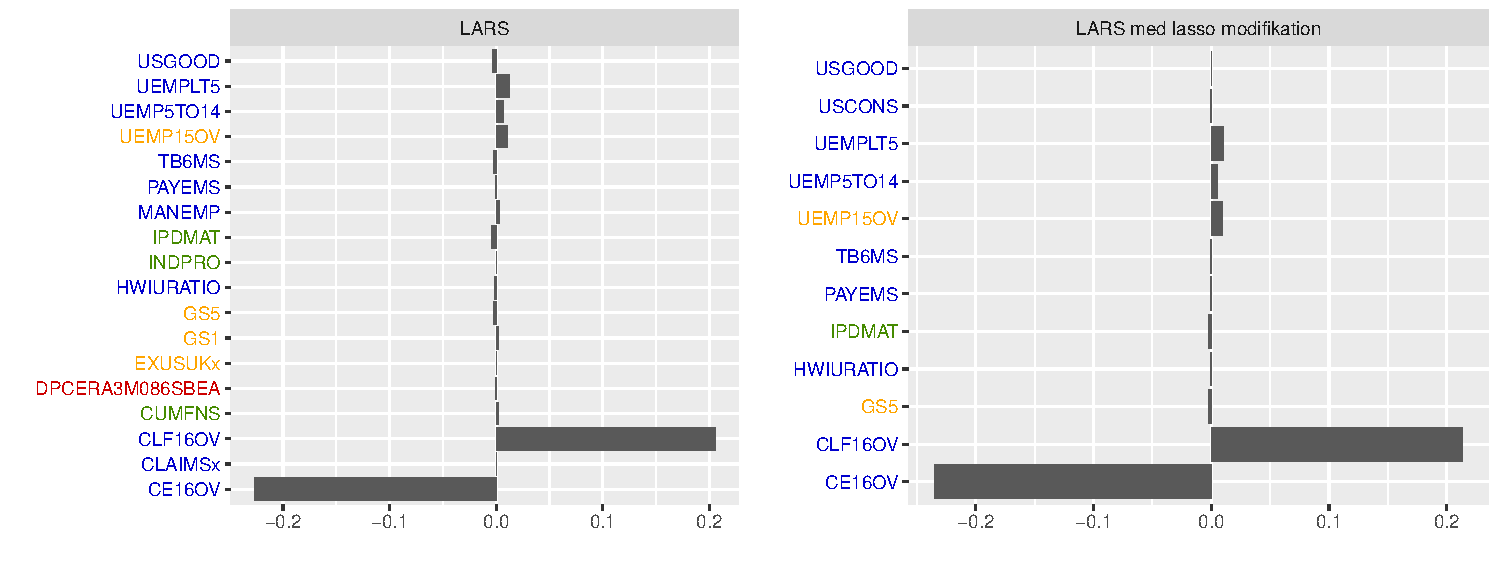
\includegraphics[width=1\linewidth, height=0.7\textheight]{slides/coef_lars_kryds.pdf}
%\caption{Estimerede koefficienter for LARS (CV) og lasso LARS (CV).}
%\end{figure}
%\begin{itemize}
%\item afviser normalitet samt at de første 10 autokorrelationer er nul
%\end{itemize}
%\end{frame}

\begin{frame}{LARS}{Krydsvalidering}
\begin{figure}
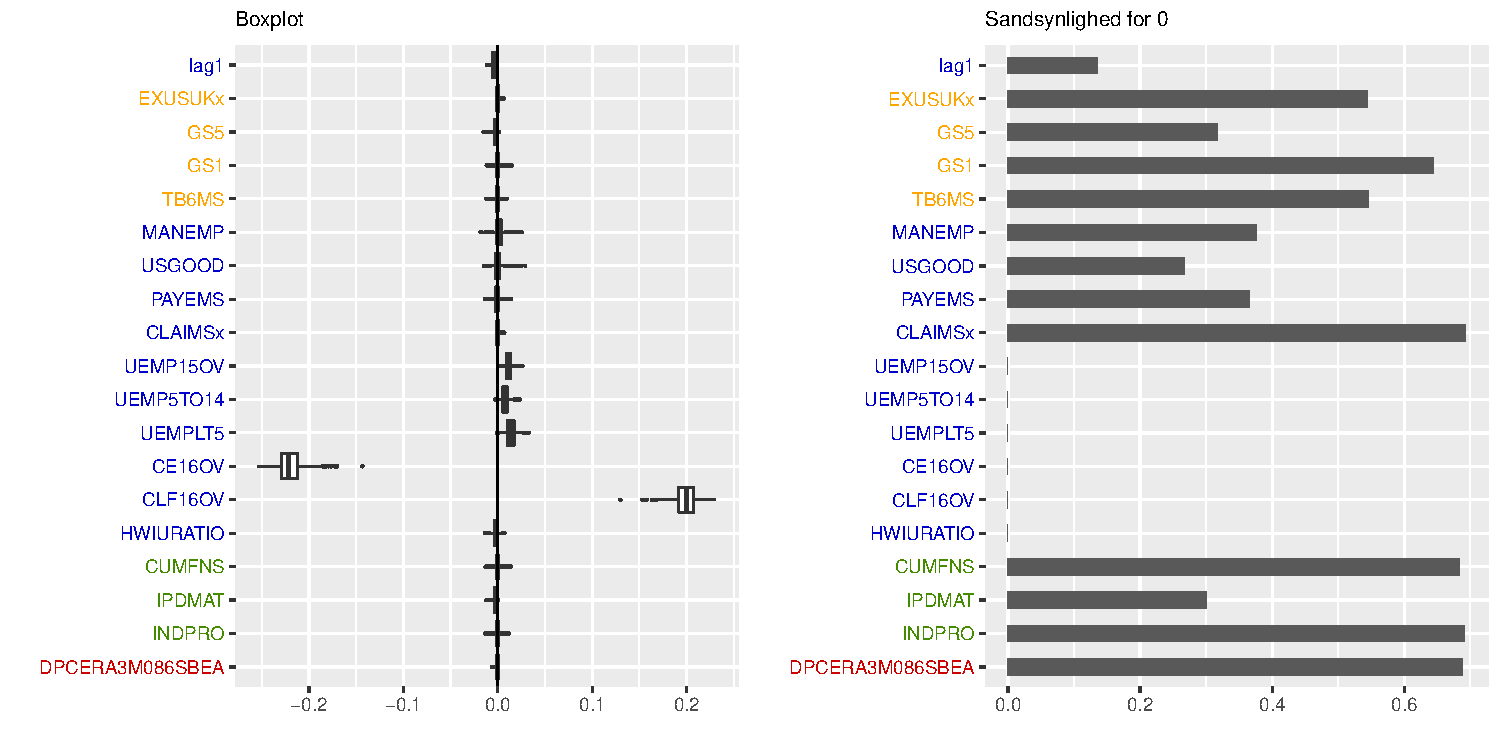
\includegraphics[width=1\linewidth, height=0.7\textheight]{slides/boxplot_lars_kryds.pdf}
\caption{Til venstre vises et boxplot af 1000 bootstrap realisationer af $\widehat{\boldsymbol{\beta}}^{\text{LARS}} \del{f_\text{1sd}} $.
Plottet til højre illustrerer andelen af bootstrap realisationer, hvor parameter estimaterne er præcis nul.}
\end{figure}
\begin{itemize}
\item afviser normalitet samt at de første 10 autokorrelationer er nul
\end{itemize}
\end{frame}

\begin{frame}{LARS}{Krydsvalidering}
\begin{figure}
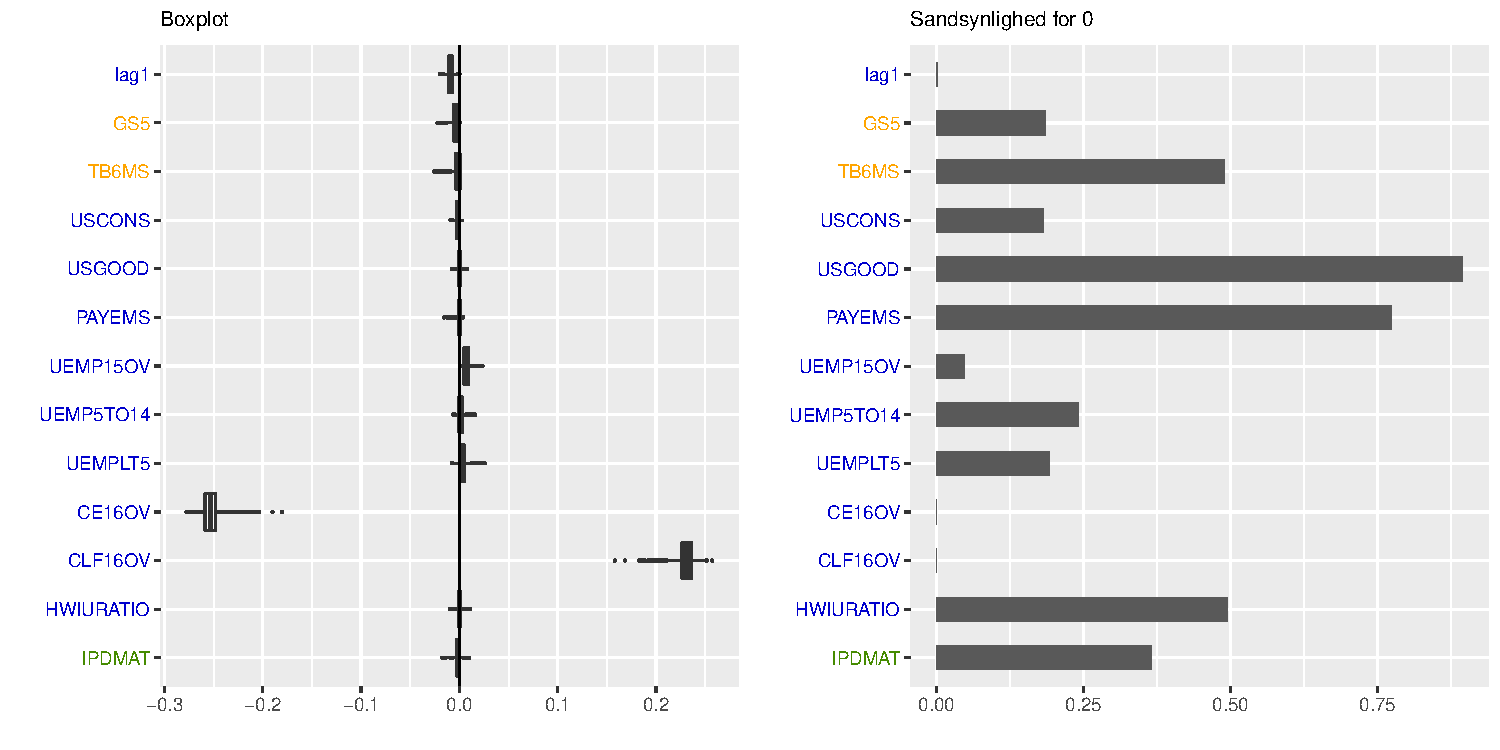
\includegraphics[width=1\linewidth, height=0.7\textheight]{slides/boxplot_lasso_kryds.pdf}
\caption{Til venstre vises et boxplot af 1000 bootstrap realisationer af $\widehat{\boldsymbol{\beta}}^{\text{lasso}} \del{f_\text{1sd}} $.
Plottet til højre illustrerer andelen af bootstrap realisationer, hvor parameter estimaterne er præcis nul.}
\end{figure}
\begin{itemize}
\item afviser normalitet samt at de første 10 autokorrelationer er nul
\end{itemize}
\end{frame}

\begin{frame}{LARS}{Krydsvalidering}
\begin{table}[ht] 
\centering 
\scalebox{0.8}{
\begin{tabular}{lccc}
%\multicolumn{3}{l}{LARS algoritmen med lasso modifikation} \\
\toprule
Prædiktor & Cov test & \(p\)-værdi \\
\midrule
 \textcolor{blue3}{HWIURATIO}  &   864.6317 & 0 \\
 \textcolor{blue3}{UEMP15OV}  &   161.3770&  0 \\
 \textcolor{blue3}{UEMPLT5} &  163.0670 & 0 \\
 \textcolor{blue3}{UEMP5TO14}  &   122.3840  &0 \\
 \textcolor{blue3}{CE16OV} & 14.7416  &0 \\
 \textcolor{blue3}{PAYEMS} &  0.3356  &0.7151 \\
  \textcolor{blue3}{USGOOD}  &   5.0872 & 0.0066 \\
 \textcolor{blue3}{CLF16OV}    &   221.9181 & 0 \\
\textcolor{chartreuse4}{IPDMAT}       &    0.0668&  0.9354 \\
\textcolor{orange}{GS5}   &       0.3856 &    0.6803 \\
 \textcolor{blue3}{ lag1 }  &      0.8897 &    0.4115 \\
\textcolor{orange}{ TB6MS }&       0.0419   &  0.9590 \\
 \textcolor{blue3}{USCONS }&   0.0132   &  0.9869 \\ 
\bottomrule
\end{tabular}}
\caption{Kovarians testen for lasso LARS (CV).
Vi viser kun \(p\)-værdier for prædiktorer som medtages og bliver i modellen, dvs hvis en prædiktor medtages i et trin og senere forlader modellen, vises denne prædiktor ikke.
\(p\)-værdier \(< 2.2 \cdot 10^{-16}\) sættes lig 0.} \label{tab:covTest}
\end{table} 
\end{frame}

\begin{frame}{LARS}{Krydsvalidering}
\begin{table}[ht] 
\centering 
\scalebox{0.6}{
\begin{tabular}{lccccccc}
%\multicolumn{9}{l}{LARS algoritmen} \\
\toprule
Prædiktor& Koefficient & Z-score &\(p\)-værdi & Konfidensinterval &   $\sbr{\pazocal{V}^-,\pazocal{V}^+}$   \\
\midrule
\textcolor{blue3}{HWIURATIO}& 0.002  & 0.694   & 0.160    &  $\del{-\infty   ,  \infty}$   &$\sbr{0.002,0.002} $    \\
 \textcolor{blue3}{UEMP15OV} &    0.004&   1.606 & 0.923 &     $ \left( -\infty  ,  0.032\right] $     &$\sbr{0.004, 0.005}$   \\
 \textcolor{blue3}{UEMPLT5} & 0.001   &0.149   & 0.064  & $ \left[-0.018  ,     \infty\right) $  & $\sbr{0.000 ,0.001}$   \\
\textcolor{blue3}{MANEMP}   &   0.002 &  0.486   &0.273 &   $\left[-0.171 ,      \infty\right)$  & $\sbr{0.002,0.003}$\\
 \textcolor{blue3}{UEMP5TO14}  &$-  0.001$ & $-0.242 $ &0.077  &   $ \left( -\infty    ,  0.016\right] $&      $\sbr{0.000 ,0.001}$ \\
\textcolor{blue3}{CE16OV} &$- 0.267$ &$-37.446$ & 0.130   &   $\left( -\infty   ,  0.532\right]  $&    $\sbr{0.267, 0.267}$     \\ 
\textcolor{blue3}{ PAYEMS } &   0.000 &  0.006  & 0.563   &  $\del{-\infty ,  \infty}$   & $\sbr{0.000 ,0.000}$  \\
 \textcolor{blue3}{USGOOD} &$- 0.003$  &$-0.498$ &0.638   &   $\del{-\infty ,  \infty}$ &    $\sbr{0.003 ,0.003}$\\
\textcolor{chartreuse4}{CUMFNS} &  0.002  & 0.404 & 0.478    & $\del{-\infty   ,  \infty}$  &  $\sbr{0.002 ,0.002 }$  \\
 \textcolor{blue3}{CLF16OV} &  0.243  &36.643   & 0.179   &  $\del{-\infty  ,  \infty}$ &  $\sbr{0.243 ,0.243}$ \\  
\textcolor{chartreuse4}{ IPDMAT}& $-0.006$ &$ -1.626 $  &0.874   & $\left[-0.125  ,    \infty\right) $& $\sbr{0.006, 0.006}$ \\   
\textcolor{orange}{ TB6MS} & $-0.005$  &$-0.715$  & 0.569 &     $\del{-\infty  ,  \infty}$&   $\sbr{0.005, 0.006}$   \\ 
\textcolor{chartreuse4}{INDPRO} &  0.003 &  0.513  &0.328   &  $\del{-\infty   ,  \infty }$    & $\sbr{0.003 ,0.003}$  \\
\textcolor{orange}{GS1} &   0.006&   0.577    &0.473  &    $\del{-\infty  ,  \infty}$  &$\sbr{0.006 ,0.006}$ \\  
\textcolor{orange}{GS5} & $-0.005$ & $-1.146 $ &0.037 &     $\left( -\infty ,  -0.025\right]   $ & $\sbr{0.005 ,0.005 }$\\  
 \textcolor{blue3}{lag1}  & $-0.009$  &$-3.949$   & 0.910   & $\del{-\infty  ,  \infty }$  &$\sbr{0.009, 0.009 }$ \\ 
 \textcolor{red3}{DPCERA3M086SBEA} & $- 0.003$ & $-1.436$ & 0.233  &   $\del{-\infty   ,  \infty }$ &  $\sbr{0.003, 0.003}$ \\ 
\textcolor{orange}{ EXUSUKx}  &  0.003   &1.383 & 0.964   &   $\left( -\infty     ,-0.053 \right] $&  $\sbr{0.003, 0.003 }$   \\   
 \textcolor{blue3}{CLAIMSx} &0.002 &  0.813   & 0.226 &    $\del{-\infty  ,  \infty}$& $\sbr{0.002 ,0.002 }$   \\ 
\bottomrule
\end{tabular}  
}
\caption{Koefficienter, \(Z\)-scores, \(p\)-værdier, konfidensintervaller og trunkeret intervaller for LARS$_{TG}$ (CV). Den estimeres standard afvigelse er \(0.043\), og resultaterne er for \(f_{1 \text{sd}} = 0.2542\) med \(\alpha = 0.1\).} \label{tab:larInf_kryds}
\end{table} 
\begin{itemize}
\item afviser normalitet samt at de første 10 autokorrelationer er nul
\end{itemize}
\end{frame}

%%%%%%%% BIC %%%%%%%%%
\subsection{BIC}
\begin{frame}{LARS}{BIC}
\begin{table}
\center
\scalebox{0.8}{
\begin{tabular}{lccccc| lccccc} 
\toprule
\multicolumn{6}{c}{LARS (BIC)}  & \multicolumn{6}{c}{Lasso LARS (BIC)} \\ \midrule
& Værdi & BIC & $p$ & R$^2_{\text{adj}}$ & LogLik& & Værdi & BIC & $p$ & R$^2_{\text{adj}}$ & LogLik \\
$f_\text{BIC}$ & 0.2623 & $-6.0925$ & 20 &94.43\% & 975.2909  &$f_\text{BIC}$ &  0.2604 &$-6.1627$& 17 &  94.46\% & 974.9938 \\ \bottomrule
 \end{tabular}}
\caption{Værdien af $f_\text{BIC}$, antallet af parametre, BIC, justeret R$^2$  og log-likelihood for LARS og lasso LARS.} \label{tab:bic_lars}
\end{table}
\begin{itemize}
\item 32 trin udføres for lasso LARS (BIC), hvor variablerne \textcolor{chartreuse4}{CUMFNS}, \textcolor{blue3}{MANEMP}, \textcolor{orange}{GS1}, \textcolor{blue3}{HWIURATIO}, \textcolor{blue3}{PAYMENS} og \textcolor{blue3}{USGOOD} tilføjes og fjernes igen og variablen \textcolor{orange}{TB6MS} bliver tilføjet, fjernet og så tilføjet igen. 
\end{itemize}
\end{frame}

%\begin{frame}{LARS}{BIC}
%\begin{figure}
% 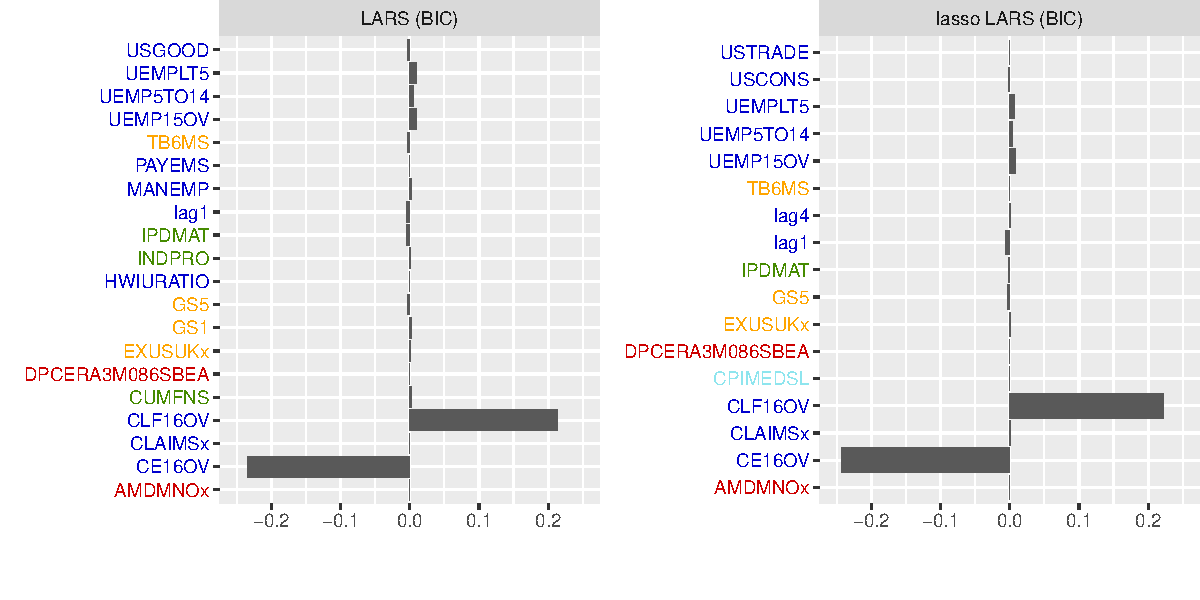
\includegraphics[width=1\linewidth, height=0.7\textheight]{slides/coef_plot_lars_bic.pdf}
% \caption{Estimerede koefficienter for LARS (BIC) og lasso LARS (BIC).}
% \end{figure}
% \begin{itemize}
%\item afviser normalitet samt at de første 10 autokorrelationer er nul
%\end{itemize}
%\end{frame}

\begin{frame}{LARS}{BIC}
\begin{figure}
 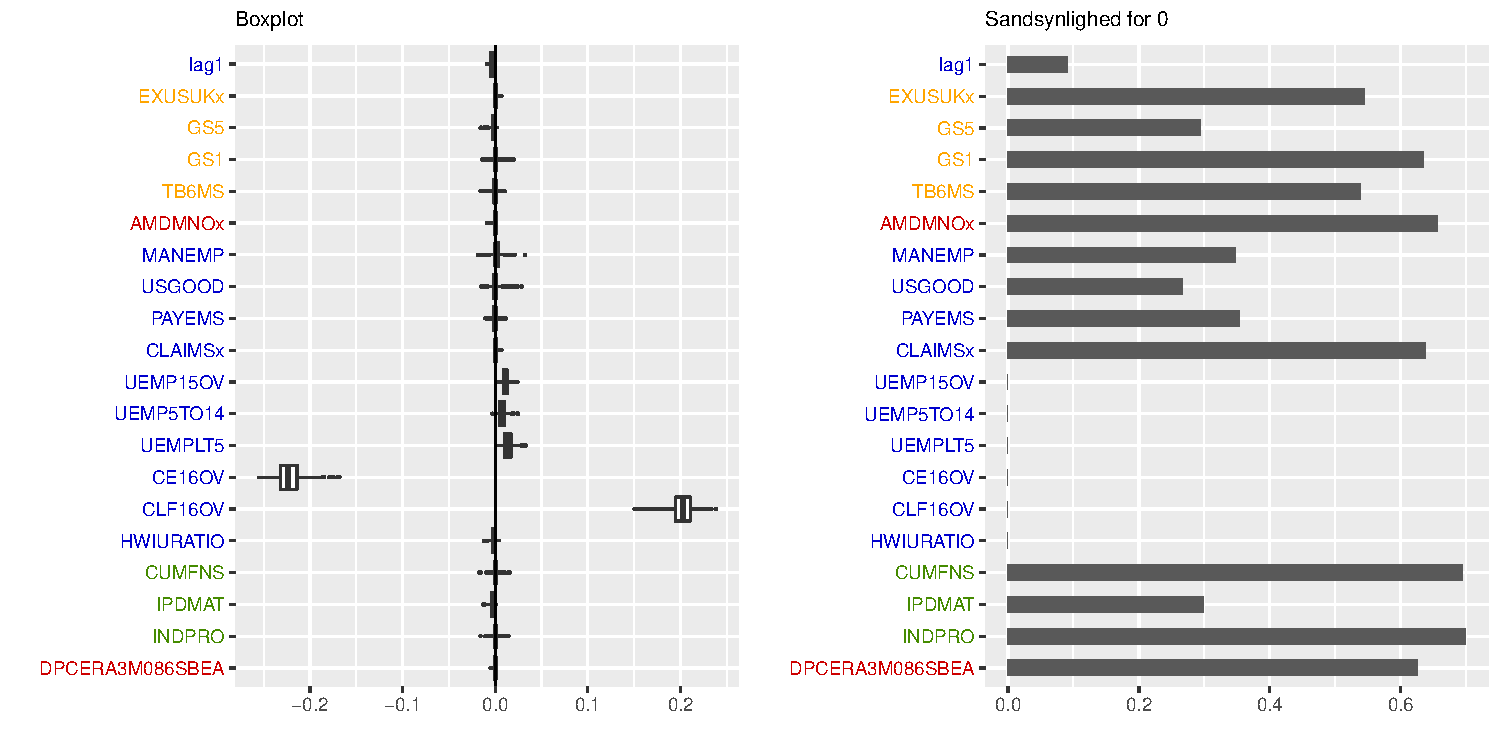
\includegraphics[width=1\linewidth, height=0.7\textheight]{slides/boxplot_lars_bic.pdf}
 \caption{Til venstre vises et boxplot af 1000 bootstrap realisationer af $\widehat{\boldsymbol{\beta}}^{\text{LARS}} \del{f_\text{BIC}} $.
Plottet til højre illustrerer andelen af bootstrap realisationer, hvor parameter estimaterne er præcis nul.}
 \end{figure}
 \begin{itemize}
\item afviser normalitet samt at de første 10 autokorrelationer er nul
\end{itemize}
\end{frame}


\begin{frame}{LARS}{BIC}
\begin{figure}
 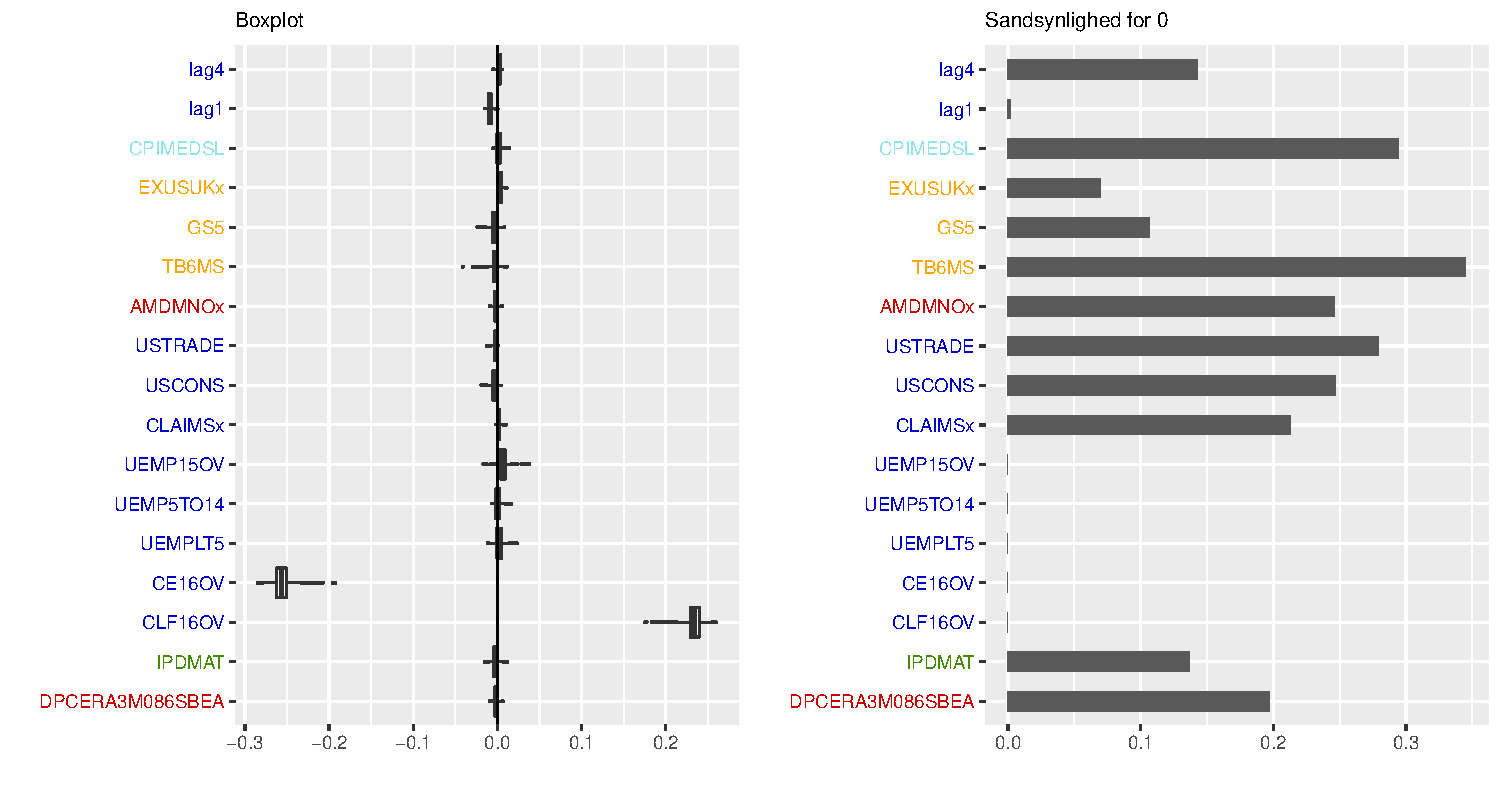
\includegraphics[width=1\linewidth, height=0.7\textheight]{slides/boxplot_lars_lasso_bic.pdf}
 \caption{Til venstre vises et boxplot af 1000 bootstrap realisationer af $\widehat{\boldsymbol{\beta}}^{\text{lasso}} \del{f_\text{BIC}} $.
Plottet til højre illustrerer andelen af bootstrap realisationer, hvor parameter estimaterne er præcis nul. }
 \end{figure}
 \begin{itemize}
\item afviser normalitet samt at de første 10 autokorrelationer er nul
\end{itemize}
\end{frame}

\begin{frame}{LARS}{BIC}
\begin{table}[ht] 
\centering 
\scalebox{0.6}{
\begin{tabular}{lccc}
%\multicolumn{3}{l}{LARS algoritmen med lasso modifikation} \\
\toprule
Prædiktor & Cov test & \(p\)-værdi \\
\midrule
\textcolor{blue3}{UEMP15OV}    &       161.3770  &0\\
\textcolor{blue3}{UEMPLT5}   &      163.0670 & 0\\
\textcolor{blue3}{UEMP5TO14}    &    122.3840&  0\\
\textcolor{blue3}{CE16OV}         &   14.7416 & 0\\
\textcolor{blue3}{CLF16OV}        &   221.9181 & 0\\
\textcolor{chartreuse4}{IPDMAT}         &    0.0668&  0.9354\\
\textcolor{orange}{GS5}&   0.3856 & 0.6803\\
\textcolor{blue3}{lag1}       &      0.8897 & 0.4115\\
\textcolor{orange}{TB6MS}  &    0.0419 & 0.9590\\
\textcolor{blue3}{USCONS} &    0.0132&  0.9869\\
\textcolor{red3}{ DPCERA3M086SBEA}          &  0.0254 & 0.9750\\
\textcolor{orange}{ EXUSUKx} &     0.2309 & 0.7939\\
\textcolor{blue3}{CLAIMSx} &      0.0082 &  0.9919\\
\textcolor{red3}{ AMDMNOx}  &     0.0464 & 0.9546\\
\textcolor{blue3}{lag4 }     &    0.2281&  0.7962\\
\textcolor{cadetblue2}{CPIMEDSL}  &   0.0719&  0.9307\\
\textcolor{blue3}{USTRADE}   &     0.0029 &  0.9971\\ \bottomrule
\end{tabular}}
\caption{Kovarians testen for lasso LARS (BIC).
Vi viser kun \(p\)-værdier for prædiktorer som medtages og bliver i modellen, dvs hvis en prædiktor medtages i et trin og senere forlader modellen, vises denne prædiktor ikke.
\(p\)-værdier \(< 2.2 \cdot 10^{-16}\) sættes lig 0.} \label{tab:covTest_bic}
\end{table} 
\end{frame}

\begin{frame}{LARS}{BIC}
\begin{table}[ht] 
\centering 
\scalebox{0.6}{
\begin{tabular}{lcccccc}
%\multicolumn{9}{l}{LARS algoritmen} \\ 
\toprule
Prædiktor&  Koefficient & Z-score  & \(p\)-værdi & Konfidensinterval& $\sbr{\pazocal{V}^-,\pazocal{V}^+}$   \\ \midrule
\textcolor{blue3}{HWIURATIO} &0.002  & 0.720   &0.161    &   $\del{-\infty   ,  \infty }$ &  $\sbr{0.002,0.002}$    \\
 \textcolor{blue3}{UEMP15OV} & 0.004  & 1.596  4 &  0.920 &     $\left( -\infty  ,      0.034 \right] $& $\sbr{0.004 ,0.005}$  \\
\textcolor{blue3}{UEMPLT5}  & 0.001 &  0.148   & 0.065  & $\left[-0.018    ,    \infty  \right)$   &$\sbr{0.000,0.001}$    \\
\textcolor{blue3}{MANEMP} &0.003 &  0.561    & 0.766 &       $\left(  -\infty     ,  0.120\right] $ &$\sbr{0.003, 0.003}$  \\
 \textcolor{blue3}{ UEMP5TO14} & 0.001 & $-0.261$ &  0.093   &  $\left( - \infty    ,  0.023\right] $&   $\sbr{0.000, 0.001}$ \\
\textcolor{blue3}{ CE16OV}   & $-0.267 $& $-37.412$  & 0.130  &    $\left( -\infty     ,   0.574\right] $  &$\sbr{0.266, 0.267}$ \\
 \textcolor{blue3}{PAYEMS} &  0.000  & 0.012  & 0.428  &    $\del{-\infty   ,  \infty }$ &  $\sbr{0.000 ,  0.000}$   \\
 \textcolor{blue3}{USGOOD} & $-0.004$ & $-0.584$ & 0.721   &   $\del{-\infty   ,  \infty } $&    $\sbr{0.004 ,  0.004   }$   \\
\textcolor{chartreuse4}{CUMFNS} &  0.002   &0.390  & 0.455     &  $\del{-\infty   ,  \infty }$& $\sbr{0.002 ,  0.002 }$   \\
 \textcolor{blue3}{ CLF16OV}  &   0.243 & 36.646   &  0.179    &  $\del{-\infty   ,  \infty }$&$\sbr{0.243 ,  0.243}$    \\
\textcolor{chartreuse4}{ IPDMAT}& $-0.006$ & $ -1.618$   & 0.869  & $\left[ -0.130  ,      \infty  \right)$&   $\sbr{0.006,   0.006}$     \\
 \textcolor{orange}{TB6MS}& $-0.006$ & $-0.790 $  & 0.615     &  $\del{-\infty   ,  \infty } $  & $\sbr{0.006 ,  0.006}$   \\
 \textcolor{chartreuse4}{INDPRO}&   0.003   &0.591   & 0.494  &    $\del{-\infty   ,  \infty }$ &  $\sbr{0.003,   0.003}$    \\
 \textcolor{orange}{GS1} &  0.007&   0.675  & 0.571 &      $\del{-\infty   ,  \infty }$ &   $\sbr{0.007 ,  0.007}$     \\
 \textcolor{orange}{GS5} &   $-0.006$ &$ -1.240$  & 0.302&      $\del{-\infty   ,  \infty }$&   $\sbr{0.006,  0.006}$   \\
 \textcolor{blue3}{lag1} & $-0.009$ & $ -3.914  $  &  0.912   &  $\del{-\infty   ,  \infty }$& $\sbr{0.009,   0.009 }$   \\
  \textcolor{red3}{DPCERA3M086SBEA}   & $-0.002$ &  $-1.331  $ & 0.225 &      $\del{-\infty   ,  \infty }$& $\sbr{0.002,   0.002 }$   \\
 \textcolor{orange}{EXUSUKx} & 0.003 &  1.357   & 0.964  &    $\left( -\infty   ,  -0.051\right] $&  $\sbr{0.003 ,  0.003}$   \\
 \textcolor{blue3}{CLAIMSx} &  0.001  & 0.629  & 0.208   &   $\del{-\infty   ,  \infty }$ & $\sbr{ 0.001 ,  0.001 }$  \\
 \textcolor{red3}{AMDMNOx} &  $-0.002$ &  $-0.904 $   & 0.855     &  $\del{-\infty   ,  \infty }$&$\sbr{0.002 ,  0.002}$  \\ \bottomrule
\end{tabular}  
}
\caption{Koefficienter, \(Z\)-scores, \(p\)-værdier, konfidensintervaller og trunkeret intervaller for LARS$_{TG}$ (BIC). Den estimeres standard afvigelse er \(0.043\), og resultaterne er for \(\widehat{f}_{\text{BIC}} = 0.2623 \) med \(\alpha = 0.1\).} \label{tab:larInf_bic}
\end{table} 
 \begin{itemize}
\item afviser normalitet samt at de første 10 autokorrelationer er nul
\end{itemize}
\end{frame}


%%% Local Variables:
%%% mode: latex
%%% TeX-master: "../beamer"
%%% End:



